\documentclass[border=1pt, 12pt, tikz]{standalone}

\newcommand\wideOne{2cm}%{3cm}
\newcommand\wideTwo{3.5cm}%{4cm}
\newcommand\wideThree{1.5cm}
\newcommand\wideFour{2cm}
\newcommand\distOne{2cm}
\newcommand\distTwo{1cm}

\begin{document}
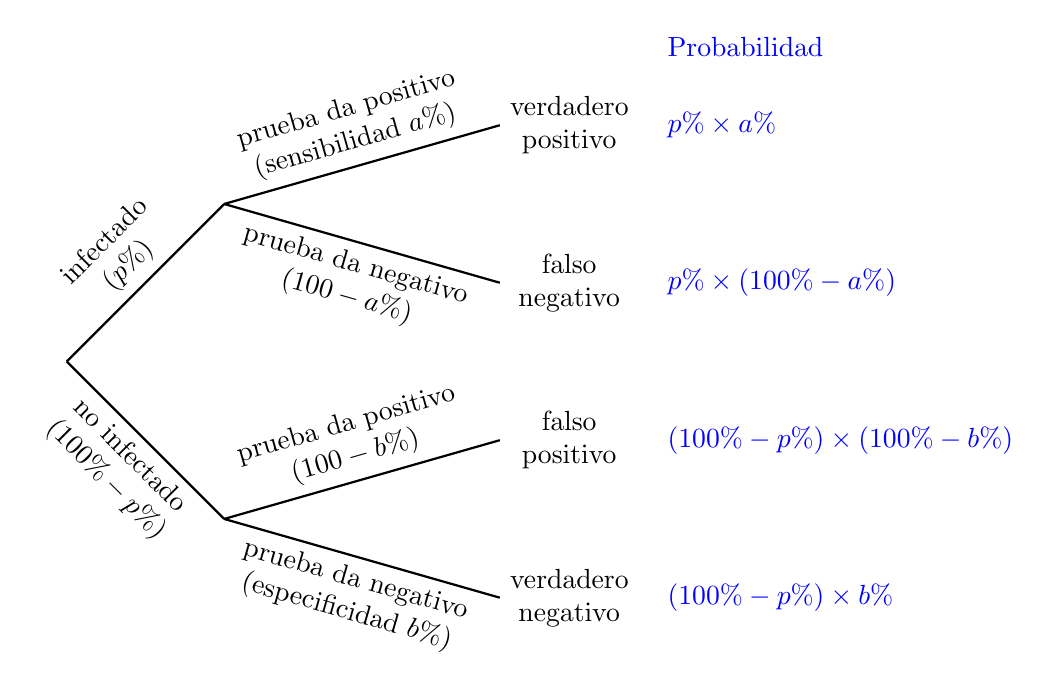
\begin{tikzpicture}[scale=1]

% 1st level
\draw[thick]%
   (0,0) 
   -- node[above, sloped, align=center]
      {infectado\\$(p\%)$}
   (\wideOne,\distOne);
\draw[thick] 
   (0,0) 
   -- node[below, sloped, align=center]
      {no infectado\\$(100\%-p\%)$} 
   (\wideOne,-\distOne);

% 2nd, 3rd and 4th Level
\draw[thick] 
   (\wideOne,\distOne)
   -- node[above, align=center, sloped]
      {prueba da positivo\\(sensibilidad $a\%$)}
   ++ (\wideTwo,\distTwo) 
      node[right, align=center, text width=\wideThree]
      {verdadero\\positivo}
   ++ (\wideFour,0) 
      node[right, blue]
      {$p\%\times a\%$}
   ++ (0,1)
      node[right]
      {\textcolor{blue}{Probabilidad}}
   ; 
\draw[thick] 
   (\wideOne,\distOne) 
   -- node[below, align=center, sloped]
      {prueba da negativo\\$(100-a\%)$}
   ++ (\wideTwo,-\distTwo) 
      node[right, align=center, text width=\wideThree]
      {falso\\negativo}
   ++ (\wideFour,0) 
      node[right, blue]
      {$p\%\times (100\%-a\%)$}
   ;
\draw[thick] 
   (\wideOne,-\distOne) 
   -- node[above, align=center, sloped]
      {prueba da positivo\\$(100-b\%)$}
   ++ (\wideTwo,\distTwo) 
      node[right, align=center, text width=\wideThree]
      {falso\\positivo}
   ++ (\wideFour,0) 
      node[right, blue]
      {$(100\%-p\%)\times (100\%-b\%)$}
   ;  
\draw[thick] 
   (\wideOne,-\distOne)
   -- node[below, align=center, sloped]
      {prueba da negativo\\(especificidad $b\%$)}
   ++ (\wideTwo,-\distTwo) 
      node[right, align=center, text width=\wideThree]
      {verdadero\\negativo}
   ++ (\wideFour,0) 
      node[right, blue]
      {$(100\%-p\%)\times b\%$}
   ; 
\end{tikzpicture}
\end{document}
